\subsection{Seleccionar una técnica de modelado}

Para este trabajo decidimos utilizar dos técnicas de modelado, J48 Decision Tree
y Multilayer Perceptron. El motivo por el que elegimos estas técnicas es porque
son algoritmos supervisados, lo cual es adecuado para el problema que intentamos
resolver, y porque estos algoritmos, al funcionar sobre principios diferentes,
reaccionan de distinta forma ante distintos tipos de datos de entrada,
permitiéndonos de esta forma compararlos, y elegir el más apropiado.
Se Aplicará cada una de estas técnicas, variando sus parámetros
para obtener mejores resultados.
La clase para estos algoritmos será el atributo \code{is\_successfull}, el cual
surgirá de aplicar una función de threshold a la cantidad de views de cada
video. Para evitar que el algoritmo tenga información relacionada directamente
con la clase, quitaremos el atributo \code{views} del set de datos para aplicar
los algoritmos.

    \subsubsection{Técnica de modelado}
      \textbf{J48 Decision Tree:} Se utilizará el algoritmo supervisado J48, el cual
      consiste en un árbol de decisión utilizado para la clasificación del set
      de datos.\\
      \textbf{Multilayer Perceptron:} Se utilizará el algoritmo supervisado
      Multilayer Perceptron, el cual consiste en una Red Neuronal del tipo
      backtracking, utilizado para la clasificación del set de datos.

    \subsubsection{Supuestos de modelado}
        Todos los datos usados para el modelado son numéricos.

\subsection{Generar el diseño de las pruebas}
    \subsubsection{Diseño de las pruebas}

      Para ambas técnicas de modelado se eligió utilizar un 70% del dataset
      como set de entrenamiento y un 30% del dataset comos set de prueba,
      elegido al azar (se mezcla al azar todo el set de pruebas y se elige el
      70% de los registros que se encuentran primero). Se escogió de esta forma
      para darle suficientes datos a la red neuronal. En total quedan 12285
      registros para prueba y 28664 registros para entrenamiento.


\subsection{Construir el modelo}
    \subsubsection{Configuración de parámetros}

      \paragraph{Arbol J48}
          Para el caso del árbol J48 debemos ajustar los parámetros de nivel de
          confianza y cantidad mínima de elementos por hoja.\\\\
          \textbf{Nivel de Confianza\\}
          Un nivel de confianza demasiado alto provocará que el algoritmo no
          desestime ninguna regla lo cual llevará a un posible overfit.\\\\
          \textbf{Cantidad mínima de Elementos por hoja\\}
          Lo mismo puede ocurrir en caso de usar un valor demasiado bajo de
          cantidad minima de elementos por hoja.\\
          Luego de Experimentar con distintos valores para cada caso, llegamos a
          los siguientes valores que nos dan los mejores resultados:\\\\
          \textbf{Confidence Level:} 0.01\\
          \textbf{Minium elements per Leaf:} 80\\\\

          Luego de varios test, notamos que el valor de Minium elements per leaf
          que mejor resultado en términos de precisión era 60, pero el árbol
          quedaba demasiado grande como para comprenderlo fácilmente. Decidimos
          subirlo a 80 para obtener un árbol razonable, perdiendo una cantidad
          despreciable de precisión. Subirlo a mas de 80 ya podaba mucho el
          árbol y generaba pérdidas de precisión importantes.\\
          De la misma forma elegimos un Confidence level de 0.01. Disminuirlo
          mas generaba una pérdida de precisión, aumentarlo nos resultaba en un
          arbol mucho mas grande.

      \paragraph{Multilayer Perceptron}
          Para el caso del Multilayer Perceptron debemos ajustar la cantidad
          hidden layers, el learning rate, el momentum, el training time y el
          decay.\\\\
          \textbf{Hidden Layers\\}
          Si se colocan demasiadas hidden layers se incrementa mucho el tiempo
          de procesamiento, y ademas se corre el riesgo de overfiting. Si se
          colocan muy pocas puede que no sean suficientes para aproximar
          correctamente la función del problema.\\\\
          \textbf{Learning Rate\\}
          El learning rate y el momentum afectan la velocidad a la que intenta
          converger el algoritmo. Un learning rate o momentum demasiado elevador
          provocaran que el algoritmo no logre encontrar un mínimo local. Un
          learning rate o momentum demasiado pequeños provocan que el algoritmo
          no logre encontrar un mínimo global.\\\\
          \textbf{Training Time\\}
          Es la cantidad de pasadas de los datos a través de la red. Aumentarlo
          debería mejorar los resultados, sin embargo incrementa el tiempo de
          procesamiento y puede provocar overfiting.\\\\
          \textbf{Decay\\}
          Si está activado El algoritmo Cambia dinámicamente el learning rate
          según los resultados anteriores. Sirve para evitar que el algoritmo
          se pase por alto los mínimos, pero aumenta el tiempo de
          procesamiento.\\\\
          Luego de Experimentar con distintos valores para cada caso, llegamos a
          los siguientes valores que nos dan los mejores resultados:\\\\
          \textbf{Hidden Layers:}\\
          \textbf{Momentum:}\\
          \textbf{Learing Rate:}\\
          \textbf{Training Time:}\\
          \textbf{Decay:}\\

    \subsubsection{Modelos}

        \paragraph{Resultados de Árbol de decisión J48:}
            \subparagraph{Matriz de confusion}

                \begin{center}
                  \begin{tabular}{||c | c | c||}
                    \hline
                    is\_successfull clasificado false & is\_successfull clasificado true & \\ [0.5ex]
                    \hline
                    10106 & 174 & Era originalmente false \\
                    \hline
                    1673 & 332 & Era originalmente true \\
                    \hline
                  \end{tabular}
                \end{center}

            \subparagraph{Resultados de la clasificación}

                \begin{center}
                  \begin{tabular}{||c | c | c||}
                    \hline
                    Elementos clasificados correctamente & 10438 & 84.9654 \% \\ [0.5ex]
                    \hline
                    Instancias clasificadas en forma incorrecta & 1847 & 15.0346 \% \\
                    \hline
                  \end{tabular}
                \end{center}

            \newpage
            \subparagraph{Arbol}

                \begin{figure}[ht]
                    \begin{adjustbox}{addcode={
                        \begin{minipage}{\width}}{
                            \caption{%
                                Arbol de decision
                                }
                        \end{minipage}},rotate=360,center}
                        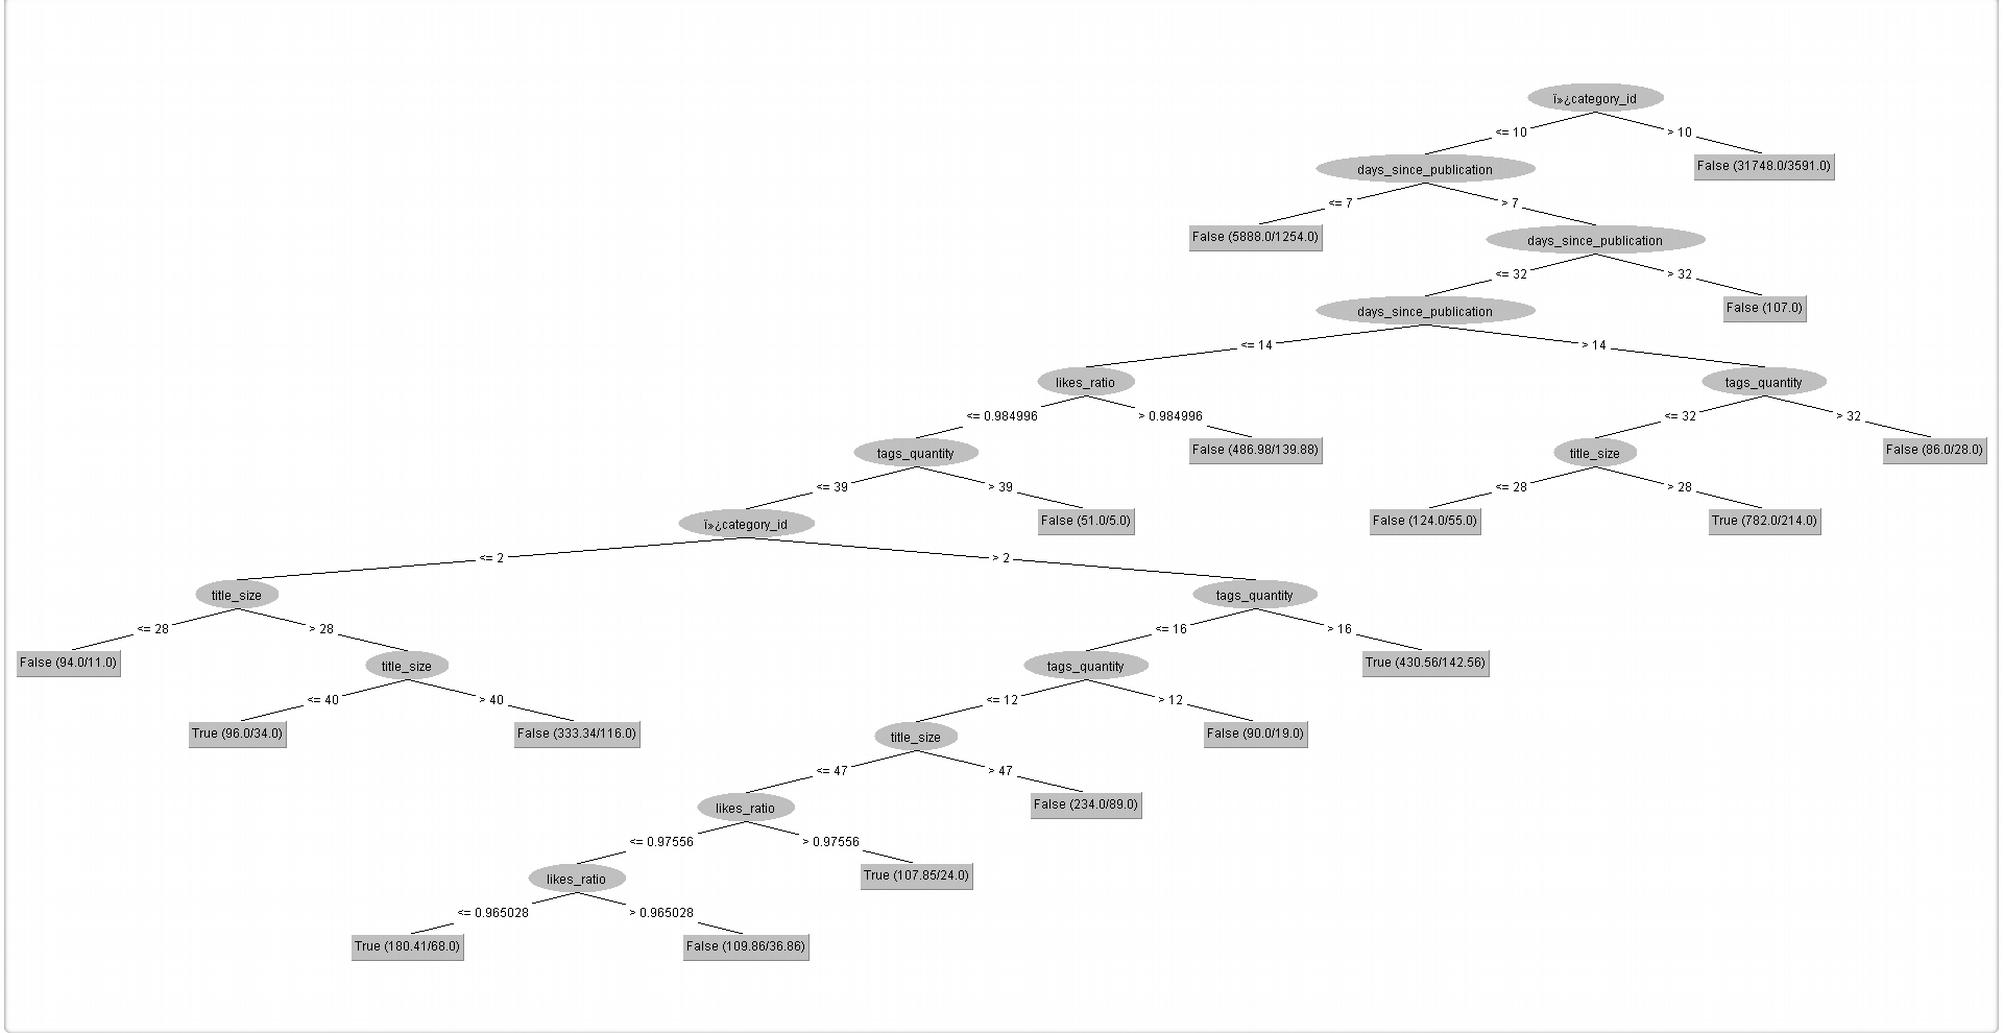
\includegraphics[scale=.4]{arbol.png}
                    \end{adjustbox}
                \end{figure}
            \FloatBarrier
            \newpage

        \subparagraph{Reglas}
            \begin{itemize}
%-------------------------------------------------------------------------------
% Regla 1
%-------------------------------------------------------------------------------
  \item Regla 1:

\begin{lstlisting}[language=bash, numbers=none]
  Si category_id <= 10
  AND days_since_publication <= 7
  Entonces
  is_successfull = false
\end{lstlisting}

  \begin{itemize}
    \item Confianza: 0.787
    \item Soporte: 0.144
    \item Captura: 0.134
  \end{itemize}

%-------------------------------------------------------------------------------
% Regla 2
%-------------------------------------------------------------------------------

  \item Regla 2:

\begin{lstlisting}[language=bash, numbers=none]
  Si category_id >= 10
  Entonces
  is_successfull = false
\end{lstlisting}

    \begin{itemize}
      \item Confianza: 0.887
      \item Soporte: 0.775
      \item Captura: 0.816
    \end{itemize}

%-------------------------------------------------------------------------------
% Regla 3
%-------------------------------------------------------------------------------
  \item Regla 3:

\begin{lstlisting}[language=bash, numbers=none]
  Si category_id <= 10
  AND days_since_publication > 7
  AND days_since_publication > 32
  Entonces
  is_successfull = false
\end{lstlisting}

    \begin{itemize}
      \item Confianza: 1
      \item Soporte: 0.003
      \item Captura: 0.003
    \end{itemize}

%-------------------------------------------------------------------------------
% Regla 4
%-------------------------------------------------------------------------------

  \item Regla 4:

\begin{lstlisting}[language=bash, numbers=none]
  Si category_id <= 10
  AND days_since_publication > 7
  AND days_since_publication <= 32
  AND days_since_publication <= 14
  AND likes_ratio > 0.985
  Entonces
  Is_successfull = False
\end{lstlisting}

    \begin{itemize}
      \item Confianza: 0.713
      \item Soporte: 0.008
      \item Captura: 0.01
    \end{itemize}

%-------------------------------------------------------------------------------
% Regla 5
%-------------------------------------------------------------------------------
  \item Regla 5:

\begin{lstlisting}[language=bash, numbers=none]
  Si category_id <= 10
  AND days_since_publication > 7
  AND days_since_publication <= 32
  AND days_since_publication > 14
  AND tags_quantity > 32
  Entonces
  is_successfull = False
\end{lstlisting}

    \begin{itemize}
      \item Confianza: 0.67
      \item Soporte: 0.0021
      \item Captura: 0.0017
    \end{itemize}

%-------------------------------------------------------------------------------
% Regla 6
%-------------------------------------------------------------------------------
  \item Regla 6:

\begin{lstlisting}[language=bash, numbers=none]
  Si category_id <= 10
  AND days_since_publication > 7
  AND days_since_publication <= 32
  AND days_since_publication > 14
  AND tags_quantity <= 32
  AND title_size <= 28
  Entonces
  is_successfull = False
\end{lstlisting}

    \begin{itemize}
      \item Confianza: 0.556
      \item Soporte: 0.003
      \item Captura: 0.002
    \end{itemize}

%-------------------------------------------------------------------------------
% Regla 7
%-------------------------------------------------------------------------------
  \item Regla 7:

\begin{lstlisting}[language=bash, numbers=none]
  Si category_id <= 10
  AND days_since_publication > 7
  AND days_since_publication <= 32
  AND days_since_publication > 14
  AND tags_quantity <= 32
  AND title_size > 28
  Entonces
  is_Successfull = True
\end{lstlisting}

    \begin{itemize}
      \item Confianza: 0.726
      \item Soporte: 0.019
      \item Captura: 0.088
    \end{itemize}

%-------------------------------------------------------------------------------
% Regla 8
%-------------------------------------------------------------------------------
  \item Regla 8:

\begin{lstlisting}[language=bash, numbers=none]
  Si category_id <= 10
  AND days_since_publication > 7
  AND days_since_publication <= 32
  AND days_since_publication <= 14
  AND likes_ratio <= 0.985
  AND tags_quantity > 39
  Entonces
  is_Successfull = False

\end{lstlisting}

    \begin{itemize}
      \item Confianza: 0.902
      \item Soporte: 0.0012
      \item Captura: 0.0013
    \end{itemize}

%-------------------------------------------------------------------------------
% Regla 9
%-------------------------------------------------------------------------------
  \item Regla 9:

\begin{lstlisting}[language=bash, numbers=none]
  Si category_id <= 10
  AND days_since_publication > 7
  AND days_since_publication <= 32
  AND days_since_publication <= 14
  AND likes_ratio <= 0.985
  AND tags_quantity < 39
  AND category_id <= 2
  AND title_size <= 28
  Entonces
  is_Successfull = False
\end{lstlisting}

    \begin{itemize}
      \item Confianza: 0.883
      \item Soporte: 0.0023
      \item Captura: 0.0024
    \end{itemize}

%-------------------------------------------------------------------------------
% Regla 10
%-------------------------------------------------------------------------------
  \item Regla 10:

\begin{lstlisting}[language=bash, numbers=none]
  Si category_id <= 10
  AND days_since_publication > 7
  AND days_since_publication <= 32
  AND days_since_publication <= 14
  AND likes_ratio <= 0.985
  AND tags_quantity < 39 & category_id <= 2
  AND title_size > 28
  AND title_size <= 40
  Entonces
  is_Successfull = True

\end{lstlisting}

    \begin{itemize}
      \item Confianza: 0.646
      \item Soporte: 0.0023
      \item Captura: 0.01
    \end{itemize}

%-------------------------------------------------------------------------------
% Regla 11
%-------------------------------------------------------------------------------
  \item Regla 11:

\begin{lstlisting}[language=bash, numbers=none]
  Si category_id <= 10
  AND days_since_publication > 7
  AND days_since_publication <= 32
  AND days_since_publication <= 14
  AND likes_ratio <= 0.985
  AND tags_quantity < 39
  AND category_id <= 2
  AND title_size > 28
  AND title_size >40
  Entonces
  is_Successfull = False
\end{lstlisting}

    \begin{itemize}
      \item Confianza: 0.652
      \item Soporte: 0.0081
      \item Captura: 0.0063
    \end{itemize}

%-------------------------------------------------------------------------------
% Regla 12
%-------------------------------------------------------------------------------
  \item Regla 12:

\begin{lstlisting}[language=bash, numbers=none]
  Si category_id <= 10
  AND days_since_publication > 7
  AND days_since_publication <= 32
  AND days_since_publication <= 14
  AND likes_ratio <= 0.985
  AND tags_quantity <= 39
  AND category_id >= 2
  AND tags_quantity > 16
  Entonces
  Is_Successfull = True
\end{lstlisting}

    \begin{itemize}
      \item Confianza: 0.67
      \item Soporte: 0.01
      \item Captura: 0.045
    \end{itemize}

%-------------------------------------------------------------------------------
% Regla 13
%-------------------------------------------------------------------------------
  \item Regla 13:

\begin{lstlisting}[language=bash, numbers=none]
  Si category_id <= 10
  AND days_since_publication > 7
  AND days_since_publication <= 32
  AND days_since_publication <= 14
  AND likes_ratio <= 0.985
  AND tags_quantity <= 39
  AND category_id >= 2
  AND tags_quantity <= 16
  AND tags_quantity > 12
  Entonces
  is_Successfull = False
\end{lstlisting}

    \begin{itemize}
      \item Confianza: 0.79
      \item Soporte: 0.0022
      \item Captura: 0.0020
    \end{itemize}

%-------------------------------------------------------------------------------
% Regla 14
%-------------------------------------------------------------------------------
  \item Regla 14:

\begin{lstlisting}[language=bash, numbers=none]
  Si category_id <= 10
  AND days_since_publication > 7
  AND days_since_publication <= 32
  AND days_since_publication <= 14
  AND likes_ratio <= 0.985
  AND tags_quantity <= 39
  AND category_id >= 2
  AND tags_quantity <= 16
  AND tags_quantity <= 12
  AND title_size > 47
  Entonces
  is_Successfull = False
\end{lstlisting}

    \begin{itemize}
      \item Confianza: 0.62
      \item Soporte: 0.0057
      \item Captura: 0.0042
    \end{itemize}

%-------------------------------------------------------------------------------
% Regla 15
%-------------------------------------------------------------------------------
  \item Regla 15:

\begin{lstlisting}[language=bash, numbers=none]
  Si category_id <= 10
  AND days_since_publication > 7
  AND days_since_publication <= 32
  AND days_since_publication <= 14
  AND likes_ratio <= 0.985
  AND tags_quantity <= 39
  AND category_id >= 2
  AND tags_quantity <= 16
  AND tags_quantity <= 12
  AND title_size <= 47
  AND likes_ratio > 0.97556
  Entonces
  is_Successfull = True
\end{lstlisting}

    \begin{itemize}
      \item Confianza: 0.776
      \item Soporte: 0.0026
      \item Captura: 0.0127
    \end{itemize}

%-------------------------------------------------------------------------------
% Regla 16
%-------------------------------------------------------------------------------
  \item Regla 16:

\begin{lstlisting}[language=bash, numbers=none]
  Si category_id <= 10
  AND days_since_publication > 7
  AND days_since_publication <= 32
  AND days_since_publication <= 14
  AND likes_ratio <= 0.985
  AND tags_quantity <= 39
  AND category_id >= 2
  AND tags_quantity <= 16
  AND tags_quantity <= 12
  AND title_size <= 47
  AND likes_ratio <= 0.97556
  AND likes_ratio <= 0.965
  Entonces
  is_Successfull = True
\end{lstlisting}

    \begin{itemize}
      \item Confianza: 0.622
      \item Soporte: 0.0044
      \item Captura: 0.017
    \end{itemize}

%-------------------------------------------------------------------------------
% Regla 17
%-------------------------------------------------------------------------------
  \item Regla 17:

\begin{lstlisting}[language=bash, numbers=none]
  Si category_id <= 10
  AND days_since_publication > 7
  AND days_since_publication <= 32
  AND days_since_publication <= 14
  AND likes_ratio <= 0.985
  AND tags_quantity <= 39
  AND category_id >= 2
  AND tags_quantity <= 16
  AND tags_quantity <= 12
  AND title_size <= 47
  AND likes_ratio <= 0.97556
  AND likes_ratio > 0.965
  Entonces
  is_Successfull = False
\end{lstlisting}

    \begin{itemize}
      \item Confianza: 0.66
      \item Soporte: 0.0027
      \item Captura: 0.0021
    \end{itemize}

\end{itemize}


        \newpage
            \subparagraph{Arbol con reglas}

            \begin{figure}[ht]
                \begin{adjustbox}{addcode={
                    \begin{minipage}{\width}}{
                        \caption{Arbol de desicion con reglas}
                    \end{minipage}},rotate=360,center}
                    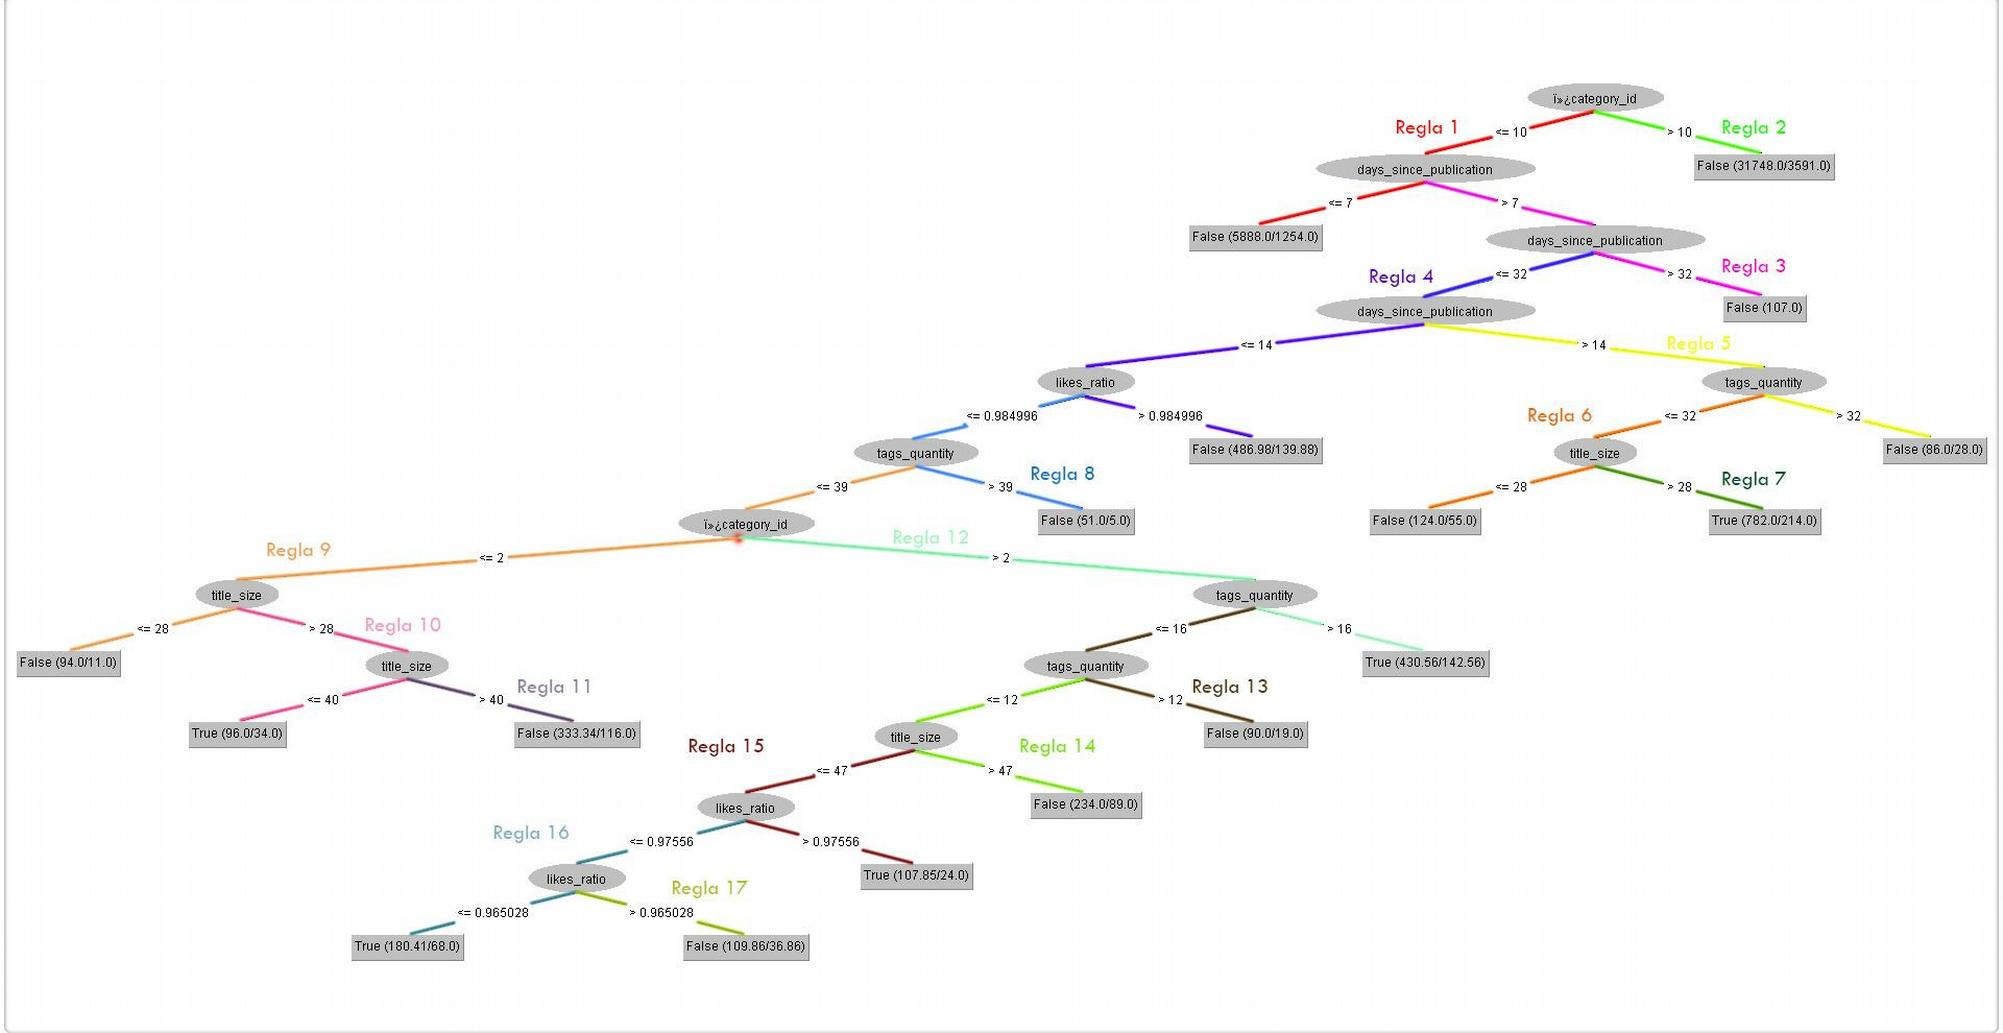
\includegraphics[scale=.4]{arbol_con_reglas.jpg}
                \end{adjustbox}
            \end{figure}
            \FloatBarrier
            \newpage

    \subsubsection{Descripción del modelo}
\subsection{Evaluar el modelo}
    \subsubsection{Evaluación del modelo}
    \subsubsection{Revisión de la configuración de parámetros}
